
%%% Local Variables:
%%% LaTeX-command: "pdflatex --shell-escape"
%%% End:

\documentclass[11pt]{article}
\usepackage[utf8]{inputenc}
\usepackage[T1]{fontenc}
\usepackage{grffile}
\usepackage{longtable}
\usepackage{wrapfig}
\usepackage{rotating}
\usepackage[normalem]{ulem}
\usepackage{amsmath}
\usepackage{textcomp}
\usepackage{amssymb}
\usepackage{capt-of}
\usepackage{hyperref}
\hypersetup{colorlinks=true, linkcolor=magenta}
\setlength{\parindent}{0in}
\usepackage[margin=0.8in]{geometry}
\usepackage[english]{babel}
\usepackage{mathtools}
\usepackage{palatino}
\usepackage{fancyhdr}
\usepackage{sectsty}
\usepackage{engord}
\usepackage{parskip}
\usepackage{minted}
\usepackage{cite}
\usepackage{graphicx}
\usepackage{subcaption}
\usepackage{setspace}
\usepackage{minted}
\usepackage[compact]{titlesec}
\usepackage{placeins}
\usepackage{color}
\usepackage{amsmath}
\usepackage{bm}
\usepackage{todonotes}
\usepackage{pdfpages}

\author{Luis Antonio Ortega Andrés}
\date{\today}
\title{Clasificación de imágenes - Transfer Learning\\\medskip
\large APRENDIZAJE PROFUNDO PARA PROCESAMIENTO DE SEÑALES DE IMAGEN Y VÍDEO}
\hypersetup{
 pdfauthor={Luis Antonio Ortega Andrés},
 pdftitle={},
 pdfkeywords={},
 pdfsubject={},
 pdflang={Spanish}}

\begin{document}

\maketitle

\section{Simple CNN}
\begin{enumerate}
    \item \emph{Tamaños de los conjuntos de entrenamiento y validación descargados del \emph{dataset} MNIST.}

        \begin{table}[H]
            \centering
            \begin{tabular}{c|cccc}
                \textbf{}     & \textbf{Alto de imagen} & \textbf{Ancho de imagen} & \textbf{Nº canales de imagen} & \textbf{Nº muestras} \\ \hline
                Entrenamiento & \( 28 \)   & \( 28 \)     &  \( 1 \)    &   \( 60.000 \)    \\
                Validación    & \( 28 \)   & \( 28 \)     &  \( 1 \)    &   \( 10.000 \)    \\
            \end{tabular}
        \end{table}
    \item \emph{Número de parámetros del modelo Simple CNN}.
        \begin{table}[H]
            \centering
            \begin{tabular}{c|c}
                           & \textbf{Nº parámetros entrenables}  \\ \hline
                Simple CNN &      \(813.802   \)                  \\
            \end{tabular}
        \end{table}

    \item \emph{Curvas de entrenamiento y validación para 10 épocas. La mejor precisión obtenida y en qué época se obtiene.}
        

        \begin{center}
            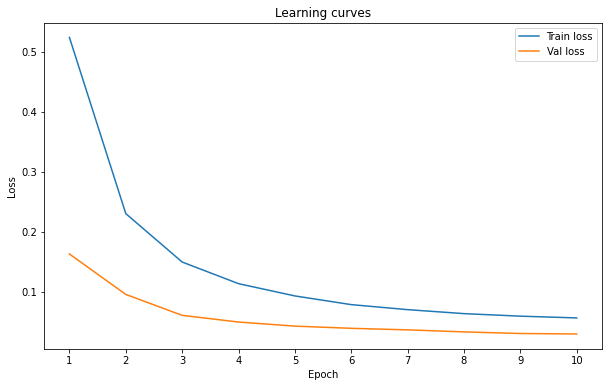
\includegraphics[scale = 0.5]{imgs/mnist_loss_curve.png}
        \end{center}
        \begin{table}[H]
            \centering
            \begin{tabular}{c|cc}
                            & \textbf{Mejor precisión (validación)} & \textbf{Época con mejor precisión} \\ \hline
                 Simple CNN &     \( 98,98 \)       &      \( 10 \)       \\
            \end{tabular}
        \end{table}
        \emph{Comentar las conclusiones sobre la evolución de la loss de entrenamiento y validación, con respecto a posibles problemas de sesgo (high-bias) o sobreajuste (overfitting). Indique si considera que continuar con más épocas de entrenamiento mejoraría el rendimiento del modelo}.

        Lo primero a notar sobre el entrenamiento del modelo, es que la función de pérdida sigue una evolución normal, donde las primeras épocas se reduce drásticamente y las últimas apenas sufre ningún cambio. Cabe destacar que la función de pérdida en el conjunto de validación es inferior al de entrenamiento, y aunque esto pueda resultar extraño, tiene sentido si tenemos en cuenta el modelo que estamos utilizando; la presencia de capas \texttt{dropout}, hace que en entrenamiento la red no disponga de toda la información que es capaz de abstraer de los datos, mientras que en validación sí que dispone de la misma.

        Respecto a la presencia de \emph{overfitting}, la evolución de las funciones de pérdida nos hace pensar que no ha sido un problema en el entrenamiento del modelo, de haberlo sido, habríamos visto como la función de perdida de entrenamiento continuaría descendiendo mientras que la de validación se mantendría constante o incluso aumentaría; lo cual no es nuestro caso.

        Por otro lado, dados los resultados y la evolución de la función de pérdida en validación, esta claro que no estamos ante un caso de \emph{underfitting}, si no que el modelo ha aprendido correctamente a diferenciar las clases dadas.

        Atendiendo al comportamiento de la pérdida en las últimas épocas, es probable que el modelo aún pueda terminar de afinar los resultados, pero no se espera que haya un cambio significativo respecto al rendimiento en la época 10. Habría que considerar si merece la pena el posible ligero aumento de rendimiento a cambio del aumento del coste computacional.


    \item \emph{Incluir la matriz de confusión obtenida. Dada esta matriz de confusión, informe de los 2 casos de confusión entre clases que ocurren con más frecuencia.}
        
        Para ilustrar mejor los resultados, la matriz de confusión ha sido calculada respecto a la cantidad de elementos de cada una de las clases, de esta forma, podemos ver cual es la pareja de clases que mas se han confundido en proporción.

        Esto puede resultar especialmente útil cuando estamos ante una base de datos muy desequilibrada, donde dar resultados de forma absoluta puede oscurecer o ensuciar el análisis.

        \begin{center}
            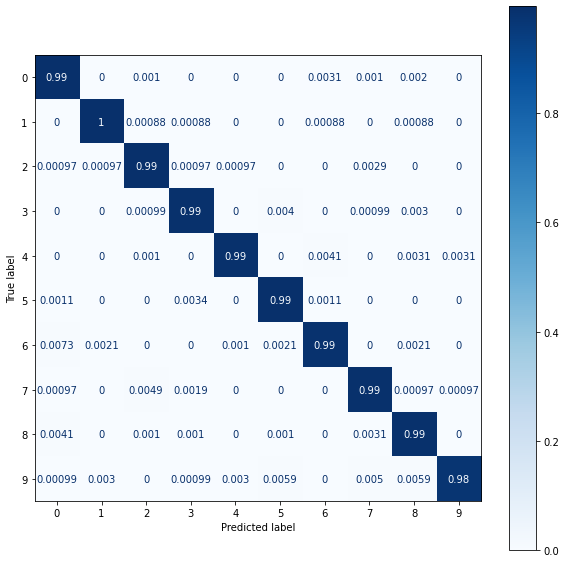
\includegraphics[scale = 0.5]{imgs/mnist_confusion_matrix.png}
        \end{center}

        En este caso, el caso de confusión más común es predecir la clase \( 0 \) cuando la clase verdadera es la clase \( 6 \). Lo cual ocurre el \( 0.73\% \) de las veces que nos encontramos con un elemento de la clase \( 6 \). Podemos ver ejemplos de este caso en la Figura~\ref{fig:1_4}.
        \begin{figure}[H]
            \centering
            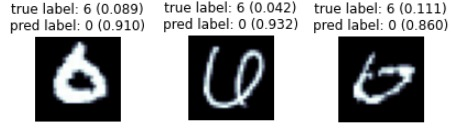
\includegraphics[scale = 0.6]{imgs/merge_wring.jpg}
            \caption{Ejemplos de confusión entre las clases \( 0 \) y \( 6 \).} \label{fig:1_4}
        \end{figure}

    \item \emph{Comente las diferencias entre el gráfico t-SNE de la representación de las capas final e intermedia de la CNN, aplicado a las imágenes del conjunto de validación. Para ello, considere la proximidad y la dispersión entre los clústeres en ambas representaciones, y su relación con la capacidad de realizar una correcta clasificación de las muestras.}
    \begin{figure}[H]
        \centering
        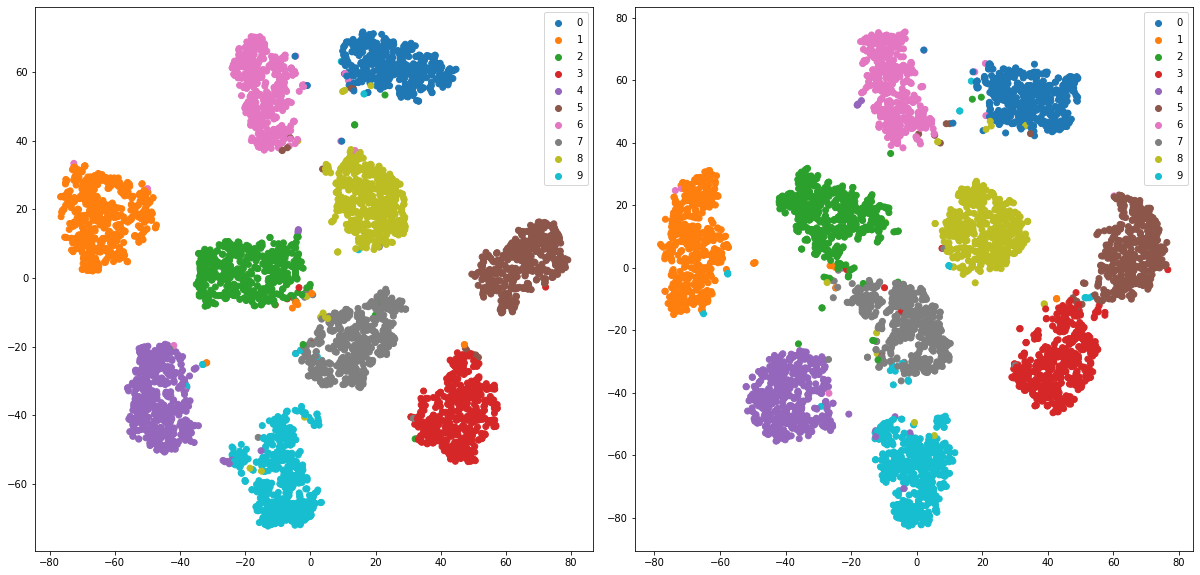
\includegraphics[scale = 0.3]{imgs/mnist_tsne.png}
        \caption{Gráficos t-SNE de la representación final (izquierda) e intermedia (derecha) de SimpleCNN.} \label{fig:1_5}
    \end{figure}

    A la vista de los resultados obtenidos en la Figura~\ref{fig:1_5}, es claro que la representación obtenida mediante t-SNE de las características en la capa final separan mejor las diferentes clases presentes en el problema que las características de las capas intermedias. En concreto, observamos lo siguiente:
    \begin{itemize}
        \item En la representación de las capas intermedias existen clases que pese a estar prácticamente separadas, se encuentran  muy próximas las unas de las otras, como es el caso de \( 3 \) y \( 5 \) o \( 2 \) y \( 7 \).
        \item En la representación de la capa final existen menos puntos en un clúster que no es el de su clase verdadera, comparado con la capas intermedias.
        \item Respecto  la dispersión de cada uno de los clusters presentes, no existe una gran diferencia entre ambas representaciones, siendo clusters de tamaño y formas muy similares.
    \end{itemize}
    A la vista de ambas representaciones, es fácil imaginar que un algoritmo de clustering como GMM o KMeans, aprendería los 10 clusters distintos sin muchos problemas, permitiendo comprobar de forma empírica la separabilidad de las representaciones (Figura~\ref{fig:1_51}).

    \begin{figure}[H]
        \centering
        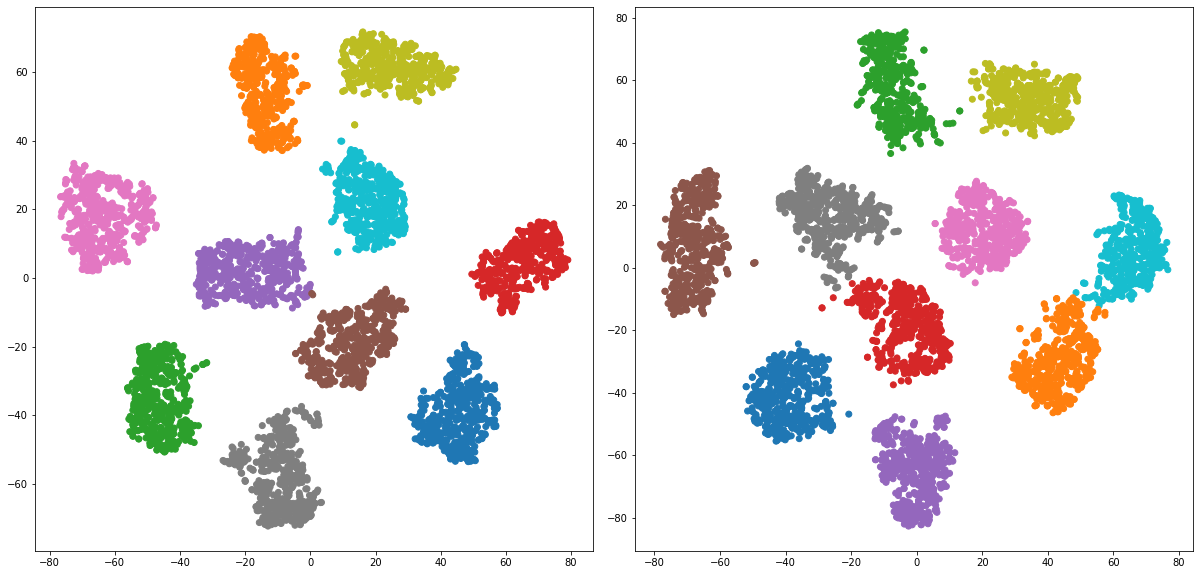
\includegraphics[scale = 0.3]{imgs/mnist_kmeans.png}
        \caption{Resultado KMeans de la representación final (izquierda) e intermedia (derecha) de SimpleCNN.} \label{fig:1_51}
    \end{figure}

\end{enumerate}
\section{AlexNet}
\begin{enumerate}
    \item \emph{Incluya el código que ha utilizado para definir la clase AlexNet}.
        \begin{minted}{python}
class AlexNet(nn.Module):
    def __init__(self, output_dim = 1):
        super(AlexNet, self).__init__()
        
        self.features = nn.Sequential(
            nn.Conv2d(3, 48, 5, 2, 2),
            nn.MaxPool2d(2),
            nn.ReLU(inplace=True),

            nn.Conv2d(48, 128, 5, 1, 2),
            nn.ReLU(inplace=True),
            nn.MaxPool2d(2),

            nn.Conv2d(128, 192, kernel_size=3, padding=1),
            nn.ReLU(inplace=True),
            nn.Conv2d(192, 192, kernel_size=3, padding=1),
            nn.ReLU(inplace=True),
            nn.Conv2d(192, 128, kernel_size=3, padding=1),
            nn.ReLU(inplace=True),
            nn.MaxPool2d(2),
        )
        
        self.classifier = nn.Sequential(
            nn.Dropout(p=0.5),
            nn.Linear(128*2*2, 2048),
            nn.ReLU(inplace=True),
            nn.Dropout(p=0.5),
            nn.Linear(2048, 2048),
            nn.ReLU(inplace=True),
            nn.Linear(2048, output_dim),
        )

    def forward(self, x):
        x = self.features(x)
        interm_features = x.view(x.shape[0], -1)
        x = self.classifier(interm_features)
        return x, interm_features
        \end{minted}

        La especificación del modelo con imágenes de entrada de dimensión \( 32 \times 32 \) es la siguiente:

        \begin{minted}{sh}
----------------------------------------------------------------
        Layer (type)               Output Shape         Param #
================================================================
            Conv2d-1           [-1, 48, 16, 16]           3,648
         MaxPool2d-2             [-1, 48, 8, 8]               0
              ReLU-3             [-1, 48, 8, 8]               0
            Conv2d-4            [-1, 128, 8, 8]         153,728
              ReLU-5            [-1, 128, 8, 8]               0
         MaxPool2d-6            [-1, 128, 4, 4]               0
            Conv2d-7            [-1, 192, 4, 4]         221,376
              ReLU-8            [-1, 192, 4, 4]               0
            Conv2d-9            [-1, 192, 4, 4]         331,968
             ReLU-10            [-1, 192, 4, 4]               0
           Conv2d-11            [-1, 128, 4, 4]         221,312
             ReLU-12            [-1, 128, 4, 4]               0
        MaxPool2d-13            [-1, 128, 2, 2]               0
          Dropout-14                  [-1, 512]               0
           Linear-15                 [-1, 2048]       1,050,624
             ReLU-16                 [-1, 2048]               0
          Dropout-17                 [-1, 2048]               0
           Linear-18                 [-1, 2048]       4,196,352
             ReLU-19                 [-1, 2048]               0
           Linear-20                   [-1, 10]          20,490
================================================================
Total params: 6,199,498
Trainable params: 6,199,498
Non-trainable params: 0
----------------------------------------------------------------
Input size (MB): 0.01
Forward/backward pass size (MB): 0.49
Params size (MB): 23.65
Estimated Total Size (MB): 24.15
----------------------------------------------------------------
        \end{minted}
    \item \emph{Número de parámetros del modelo AlexNet}.
        \begin{table}[H]
            \centering
            \begin{tabular}{c|c}
                           & \textbf{Nº parámetros entrenables}  \\ \hline
                AlexNet &      \(6,199,498   \)                  \\
            \end{tabular}
        \end{table}

    \item \emph{Incluya las curvas de entrenamiento y validación para 15 épocas. Indique también la mejor     precisión obtenida, y en qué época se logra este resultado}.
        \begin{center}
            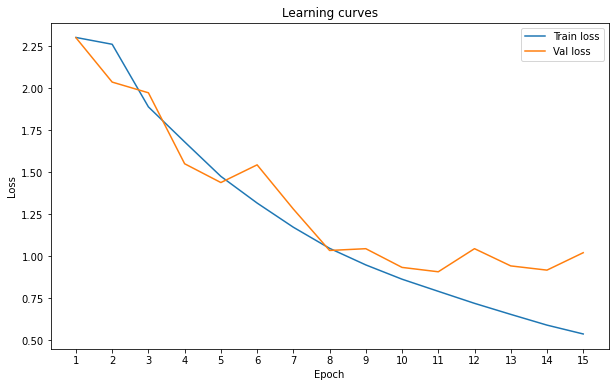
\includegraphics[scale = 0.5]{imgs/cifar_loss_curve.png}
        \end{center}
        \begin{table}[H]
            \centering
            \begin{tabular}{c|cc}
                            & \textbf{Mejor precisión (validación)} & \textbf{Época con mejor precisión} \\ \hline
                 AlexNet &     \( 0.7065 \)       &    \( 14 \)        \\
            \end{tabular}
        \end{table}
        \emph{Comentar las conclusiones sobre la evolución de la loss de entrenamiento y validación, y comentar lo que posiblemente está sucediendo después de la época 10. Indique si considera que continuar con más épocas de entrenamiento mejoraría el rendimiento del modelo.}

        En este caso, vemos como la evolución de las funciones de pérdida no es tan \emph{suave} como la que obtuvimos en el apartado anterior, especialmente en el conjunto de validación. 

        Podemos distinguir dos fases distintas en el aprendizaje:
        \begin{enumerate}
            \item \emph{Fases 1-10}: ambas funciones de pérdida disminuyen consistentemente. La pérdida en validación es más inestable, pero esto es comprensible debido a que la complejidad del problema es superior a la de MNIST.
            \item \emph{Fases 10-15}: la función de pérdida en entrenamiento disminuye consistentemente mientras que la de validación se mantiene e incluso se incrementa ligeramente en la última época. Estamos ante un claro caso de \emph{overfitting}.
        \end{enumerate}
        En este caso, incrementar el número de épocas de entrenamiento resultaría en un acentuamiento del \emph{overfitting} ya existente en el modelo, alejando el modelo del objetivo principal, que es aprender a distinguir los distintos elementos de las imágenes; y haciendo que el modelo aprenda simplemente el conjunto de entrenamiento.


    \item \emph{Incluir la matriz de confusión. Comentar los resultados obtenidos atendiendo a las características de las imágenes de cada clase.}
        \begin{center}
            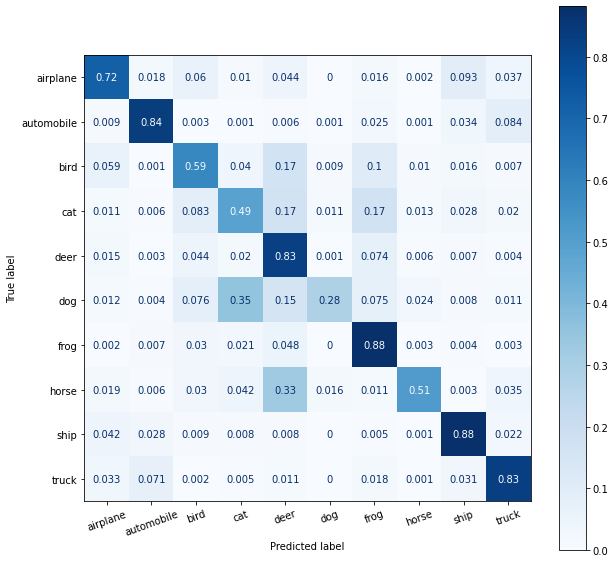
\includegraphics[scale = 0.5]{imgs/cifar_confusion_matrix.png}
        \end{center}
        
        En este caso obtenemos resultados peores comparados con los obtenidos en MNIST, como podemos ver, existen clases que se confunden más que se aciertan, como la correspondiente a \emph{dog}. Concretamente esta clase se confunde con \emph{cat} más veces de las que se etiqueta correctamente. Esto tiene sentido si tenemos en cuenta el tamaño y forma de dichos animales, pues es mas fácil confundir estos dos que un \emph{perro} y un \emph{coche}.

        Algo similar sucede con las clases \emph{horse} y \emph{deer}, que tienen una proporción de confusión del primero con el segundo de \( 0.33 \). Nuevamente esto tiene sentido debido a la naturaleza y características morfológicas de los elementos de estas clases.

        Por otro lado, otras clases como \emph{cat} y \emph{bird}, que no tienen una alta tasa de clasificación correcta, pero tampoco existe una clase predominante con la que se confundan, si no que se encuentra repartido entre las clases \emph{deer} y \emph{frog}.

    \item \emph{Incluya los resultados t-SNE para la capa última capa de la red: analice estos resultados (proximidad, dispersión, agrupación de clústeres) teniendo en cuenta la apariencia de las imágenes de las diferentes clases, sus características típicas y compare los resultados con los resultados t-SNE en el dataset MNIST.}
    
    En este caso no obtenemos clústers tan diferenciados como el caso de MNIST. Ahora, los clusters están más juntos entre sí y más dispersos y solapados. En concreto, los elementos de las clases que mas se confunden, \emph{dog} y \emph{cat} se encuentran extremadamente repartidos por todo el espacio, como cabría esperar. Algo parecido ocurre con las clases \emph{bird} y \emph{airplane}, y \emph{automobile} y \emph{truck}, que se encuentran muy mezcladas entre sí. Este comportamiento, entra dentro del esperado, pues no solo estas parejas de elementos tienen características morfológicas similares, si no que el ambiente en el que se toman las diapositivas de los mismos son parecidos, por ejemplo, en fotos de pájaros y aviones será común que el fondo corresponda con el cielo.

    Aún con todo lo anterior, las clases si se encuentran relativamente separadas y podemos ver como los clusters aprendidos por KMeans se asemeja al agrupamiento de etiquetas verdadero (Figura~\ref{fig:cifar_kmean}).

    \begin{figure}[H]
        \centering
        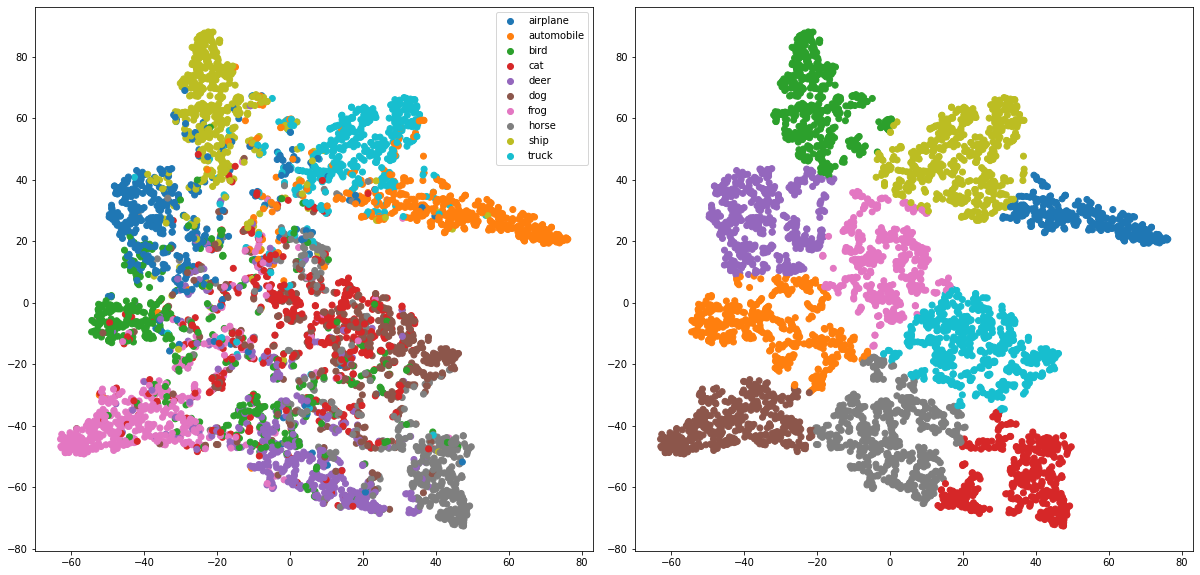
\includegraphics[scale = 0.4]{imgs/cifar.png}
        \caption{Representación t-SNE (izquierda) y resultado KMeans (derecha).}
        \label{fig:cifar_kmean}
    \end{figure}
    
\end{enumerate}
\section{Transfer Learning}

\begin{enumerate}
    \item \emph{Precisiones obtenidas para las diferentes alternativas analizadas:}
        \begin{table}[H]
            \centering
            \begin{tabular}{c|cccc}
                            & \textbf{Entren. desde cero} & \textbf{Pre-entren. + SVM} & \textbf{Fine Tunning} & \textbf{Data Aug. + Fine tunning} \\ \hline
                 Precisión & \( 0.715 \)  & \( 0.905 \)  & \( 0.915 \)  &  \( 0.965 \)         \\
            \end{tabular}
        \end{table}
    \item \emph{Compare las representaciones t-SNE de las diferentes alternativas: entrenamiento desde cero, preentrenamiento + SVM, ajuste fino (sin data augmentation) y ajuste fino (con data augmentation). A partir de las diferentes representaciones obtenidas, comente sus diferencias en cuanto a la capacidad de separar linealmente ambas clases en las cuatro alternativas analizadas.}
    
    En la Figura~\ref{fig:tsne}, podemos ver las 4 representaciones obtenidas por cada una de las técnicas aplicadas al conjunto de datos. Además, podemos ver el hiperplano separador de ambas clases aprendido mediante un SVM lineal (las puntuaciones obtenidas por el SVM se pueden ver en la Tabla~\ref{tab:svm}).

    Comentamos cada uno de los resultados obtenidos:
    \begin{itemize}
        \item \emph{Entrenamiento desde cero}. En este caso, en la representación obtenida no se aprencian clusters diferenciados de cada una de las dos clases consideradas. De esta forma, el hiperplano aprendido no llega a separar ambas clases correctamente, vemos por lo tanto que en esta representación los datos son \emph{no linealmente separables}.
        \item \emph{Pre-entrenado}. En este caso, pese a que la representación se caracteriza por una única bola, los puntos se encuentran agrupados en sus calses, obteniendo un resultado de separabilidad lineal bastante superior. De todas formas, es claro que ambas clases no llegan a ser totalmente distinguibles mediante un modelo lineal. Tanto en este método como en el anterior, la utilización de t-SNE + SVM lineal proporciona un método de clasificación muy inferior al obtenido al utilizar las redes profundas.
        \item \emph{Fine tunning y fine tunning + data augmentation}. En estos dos casos, la separabilidad de los datos es casi perfecta y evidente a simple vista, quedando planos separadores casi perfectos para ambos métodos. Podemos descatar que el resultado obtenido por el SVM linear es casi tan bueno como el obtenido por los modelos profundos completos originales, siendo que quizá si optimizaramos los parámetros del SVM podríamos equipararlos. 
    \end{itemize}

    \begin{table}[H]
        \centering
        \begin{tabular}{c|cccc}
                        & \textbf{Entren. desde cero} & \textbf{Pre-entren.} & \textbf{Fine Tunning} & \textbf{Data Aug. + Fine tunning} \\ \hline
            Separación & \( 0.585 \)  & \( 0.795 \)  & \( 0.905 \)  &  \( 0.95 \)         \\
        \end{tabular}
        \caption{Resultados de separabilidad lineal tras t-SNE.}\label{tab:svm}
    \end{table}

    \begin{figure}
        \centering
        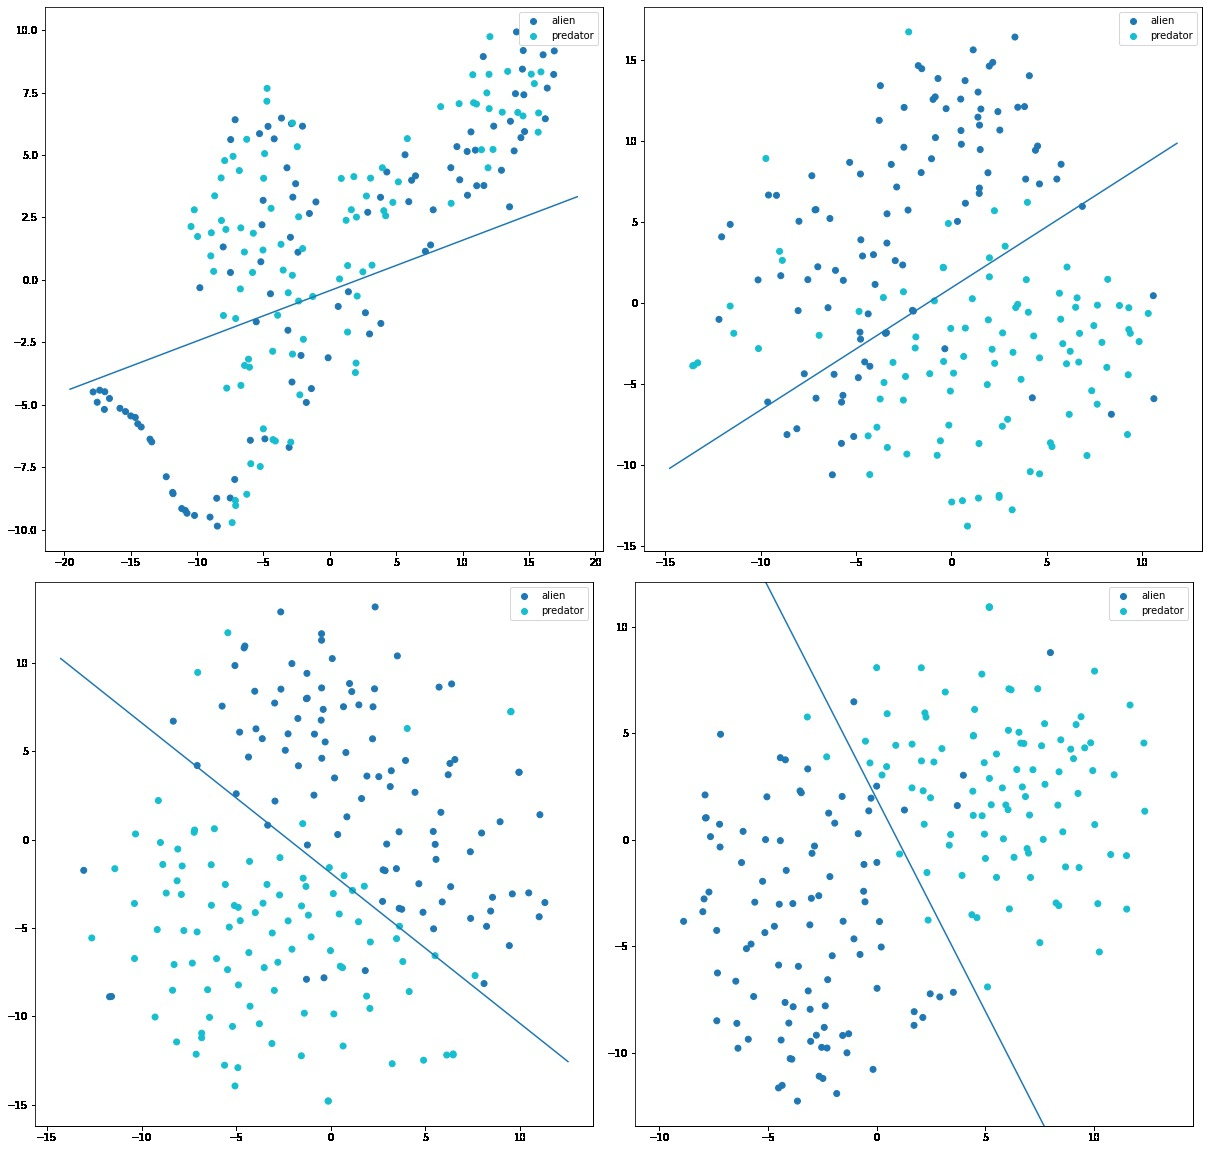
\includegraphics[scale = 0.3]{imgs/tsne.png}
        \caption{t-SNE e hiperplano separador con SVM de entrenamiento desde cero (arriba izquierda), red pre-entrenada (arriba derecha), fine tunning (abajo izquierda) y data augmentation + fine tunning (abajo derecha).}\label{fig:tsne}
    \end{figure}

    \end{enumerate}
\end{document}